% Cálculo Básico - folha estilo Stewart (derivadas, integrais, limites, trig)
\section{Cálculo I}

\begin{multicols*}{3}

\calcbox[BrickRed]{}{Limites e L'Hôpital}{
\textbf{Limites fundamentais} \\
$\lim_{x\to 0} \dfrac{\sin x}{x} = 1$ \\[0.6em]
$\lim_{x\to 0} \dfrac{e^x - 1}{x} = 1$ \\[0.6em]
$\lim_{x\to 0} \dfrac{\ln(1+x)}{x} = 1$ \\[0.6em]
$\lim_{x\to 0} (1+x)^{1/x} = e$ \\[0.6em]
$\lim_{x\to 0} \dfrac{1-\cos x}{x^2} = \dfrac{1}{2}$ \\[0.6em]
$\lim_{x\to \infty} \left(1+\dfrac{a}{x}\right)^{x} = e^{a}$ \\[0.6em]
\textbf{Regra de L'Hôpital} \\
Se $\dfrac{0}{0}$ ou $\dfrac{\infty}{\infty}$, então $\displaystyle\lim \dfrac{f}{g} = \displaystyle\lim \dfrac{f'}{g'}$ (se existir).
}

% \columnbreak

\calcbox[BrickRed]{}{Derivadas}{ 
\textbf{Regras básicas} \\ 
$\dfrac{d}{dx} c = 0$ \\[0.4em]
$\dfrac{d}{dx}[cf(x)] = cf'(x)$ \\[0.4em]
$\dfrac{d}{dx}[f\pm g] = f' \pm g'$ \\[0.5em]
$\dfrac{d}{dx}[fg] = f'g + fg'$ \\[0.6em]
$\dfrac{d}{dx}\left[\dfrac{f}{g}\right] = \dfrac{f'g - fg'}{g^2}$ \\[0.8em]
\textbf{Potência/Exp/Log} \\ 
$\dfrac{d}{dx} x^n = nx^{n-1}$ \\[0.4em]
$\dfrac{d}{dx} e^x = e^x$ \\[0.4em]
$\dfrac{d}{dx} a^x = a^x \ln a$ \\[0.4em]
$\dfrac{d}{dx} \ln x = \dfrac{1}{x}$ \\[0.6em]
\textbf{Trigonométricas} \\ 
$\dfrac{d}{dx}\sin x = \cos x$ \\[0.4em]
$\dfrac{d}{dx}\cos x = -\sin x$ \\[0.4em]
$\dfrac{d}{dx}\tan x = \sec^2 x$ \\[0.4em]
$\dfrac{d}{dx}\cot x = -\csc^2 x$ \\[0.6em]
\textbf{Inversas e Hiperbólicas} \\ 
$\dfrac{d}{dx}\arcsin x = \dfrac{1}{\sqrt{1-x^2}}$ \\[0.4em]
$\dfrac{d}{dx}\arccos x = -\dfrac{1}{\sqrt{1-x^2}}$ \\[0.4em]
$\dfrac{d}{dx}\arctan x = \dfrac{1}{1+x^2}$ \\[0.4em]
$\dfrac{d}{dx}\sinh x = \cosh x$ \\[0.4em]
$\dfrac{d}{dx}\cosh x = \sinh x$ 
}

\columnbreak

\calcbox[RoyalBlue]{}{Integrais}{
\textbf{Básicas} \\ 
$\int k\,dx = kx + C$ \\[0.4em]
$\int x^n dx = \dfrac{x^{n+1}}{n+1} + C \ (n \neq -1)$ \\[0.6em]
$\int \dfrac{1}{x} dx = \ln|x| + C$ \\[0.6em]
\textbf{Exponenciais} \\ 
$\int e^x dx = e^x + C$ \\[0.4em]
$\int a^x dx = \dfrac{a^x}{\ln a} + C$ \\[0.6em]
\textbf{Trigonométricas} \\ 
$\int \sin x dx = -\cos x + C$ \\[0.4em]
$\int \cos x dx = \sin x + C$ \\[0.4em]
$\int \tan x dx = \ln|\sec x| + C$ \\[0.6em]
$\int \sec^2 x dx = \tan x + C$ \\[0.4em]
$\int \csc^2 x dx = -\cot x + C$ \\[0.4em]
$\int \sec x\tan x dx = \sec x + C$ \\[0.6em]
\textbf{Racionais e especiais} \\ 
$\int \dfrac{1}{a^2+x^2} dx = \dfrac{1}{a}\arctan\left(\dfrac{x}{a}\right) + C$ \\[0.4em]
$\int \dfrac{1}{\sqrt{a^2-x^2}} dx = \arcsin\left(\dfrac{x}{a}\right) + C$ \\[0.4em]
$\int \dfrac{1}{x^2-a^2} dx = \dfrac{1}{2a}\ln\left|\dfrac{x-a}{x+a}\right| + C$ \\[0.6em]
$\int \sqrt{a^2-x^2} dx = \dfrac{x}{2}\sqrt{a^2-x^2} + \dfrac{a^2}{2}\arcsin\left(\dfrac{x}{a}\right) + C$ 
}

\calcbox[BrickRed]{}{Matemática Básica}{
\textbf{Fatoração} \\
$(a\pm b)^2 = a^2 \pm 2ab + b^2$ \\[0.6em]
$a^2-b^2=(a+b)(a-b)$ \\[0.6em]
$a^3\pm b^3=(a\pm b)(a^2\mp ab + b^2)$ \\[0.6em]
\textbf{Logaritmos} \\
$\ln(ab)=\ln a + \ln b$ \\[0.6em]
$\ln(a^b)=b\ln a$ \\[0.6em]
$\ln\left(\dfrac{a}{b}\right)=\ln a -\ln b$ \\[0.6em]
$e^{\ln a}=a$ 
}

% \columnbreak

\calcbox[TealBlue]{}{Círculo Trigonométrico}{
\centering
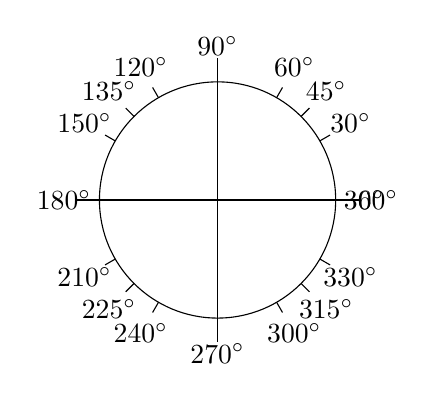
\begin{tikzpicture}[scale=1.5]
\draw (0,0) circle (1);
\draw (-1.2,0) -- (1.2,0);
\draw (0,-1.2) -- (0,1.2);
\foreach \angle in {0,30,45,60,90,120,135,150,180,210,225,240,270,300,315,330,360} {
    \draw (\angle:1) -- (\angle:1.1);
    \node at (\angle:1.3) {$\angle^\circ$};
}
\end{tikzpicture}

% Valores notáveis em tabela (mantido para clareza)
\begin{tabular}{|c|c|c|c|}
\hline
Ângulo & $\sin$ & $\cos$ & $\tan$ \\
\hline
$0^\circ$ & 0 & 1 & 0 \\
$30^\circ$ & $\tfrac{1}{2}$ & $\tfrac{\sqrt{3}}{2}$ & $\tfrac{1}{\sqrt{3}}$ \\
$45^\circ$ & $\tfrac{\sqrt{2}}{2}$ & $\tfrac{\sqrt{2}}{2}$ & 1 \\
$60^\circ$ & $\tfrac{\sqrt{3}}{2}$ & $\tfrac{1}{2}$ & $\sqrt{3}$ \\
$90^\circ$ & 1 & 0 & -- \\
$120^\circ$ & $\tfrac{\sqrt{3}}{2}$ & $-\tfrac{1}{2}$ & $-\sqrt{3}$ \\
$180^\circ$ & 0 & -1 & 0 \\
\hline
\end{tabular}
\normalsize
} 

\calcbox[RoyalBlue]{}{Trigonometria}{
\textbf{Fundamentais} \\
$\sin^2 x + \cos^2 x = 1$ \\[0.6em]
$1 + \tan^2 x = \sec^2 x$ \\[0.6em]
\textbf{Recíprocas} \\
$\dfrac{1}{\cos x} = \sec x$ \\[0.6em]
$\dfrac{1}{\sin x} = \csc x$ \\[0.6em]
\textbf{Soma/Subtração} \\
$\sin(x \pm y) = \sin x\cos y \pm \cos x\sin y$ \\[0.6em]
$\cos(x \pm y) = \cos x\cos y \mp \sin x\sin y$ \\[0.6em]
\textbf{Duplicação} \\
$\sin(2x) = 2\sin x\cos x$ \\[0.6em]
$\cos(2x) = \cos^2 x - \sin^2 x$ \\	[0.6em] 					
$\cos(2x) = 2\cos^2 x - 1$ \\[0.4em]
$\cos(2x) = 1 - 2\sin^2 x$
}

\calcbox[RoyalBlue]{}{Constantes Úteis}{
$\pi = 3{,}14159\dots$ \\[0.6em]
$e = 2{,}71828\dots$ \\[0.6em]
}

\end{multicols*}